% ready June 10, 2010

\documentclass[12pt]{article}

\setlength{\oddsidemargin}{-.5in} \setlength{\topmargin}{-.55in}
\setlength{\textwidth}{6.9in} \setlength{\textheight}{9.2in}

\usepackage{amsmath,amsthm,amssymb,amsopn,amsfonts}
\usepackage{graphics}
\usepackage{graphicx}

\newcommand{\onespace}{\renewcommand{\baselinestretch}{1}\normalsize}
\newcommand{\twospace}{\renewcommand{\baselinestretch}{1.3}\normalsize}
\newcommand{\Sobs}{{\mathcal{S}_{\mbox{\tiny{obs}}}}}
\newcommand{\Pry}{\mathbb{P}}
\newcommand{\ngood}{n_{\textup{exec}}}
\newcommand{\Y}{{\mathcal Y}}
\newcommand{\UU}{{\mathcal U}}
\newcommand{\ve}{\textup{Vec}}
\newcommand{\R}{\mathbb{R}}
\newcommand{\Z}{\mathbb{Z}}
\newcommand{\tr}{\textup{trace}}
\newcommand{\ie}{{\it i.e.\ }}
\newcommand{\mqed}{$\qed$ \medskip}

\newtheorem{theorem}{Theorem}
\newtheorem{definition}[theorem]{Definition}
\newtheorem{note}[theorem]{Note}
\newtheorem{proposition}[theorem]{Proposition}
\newtheorem{lemma}[theorem]{Lemma}
\newtheorem{corollary}[theorem]{Corollary}
\newtheorem{conjecture}[theorem]{Conjecture}
\newtheorem{keyobservation}[theorem]{Key Observation}
\newtheorem{exercise}[theorem]{Exercise}
\graphicspath{{./../graphs/}{./graphs/}}
\twospace

\begin{document}

{\Large Donniell's informal notes on Vertex Correspondence+Sancar's JOFC and rQAP2 solutions to VC. This is work in progress.}

\section{seeded graphmatch problem formulation}
Suppose $G_1$ and $G_2$ are simple graphs with respective
vertex sets $V_1$ and $V_2$, and we are given
{\it seeds} $W_1 \subset V_1$ and $W_2 \subset V_2$ such that
$|W_1|=|W_2|$, and we are given a bijective {\it seed function}
$\phi':W_1 \rightarrow W_2$.
The {\it Seeded Graphmatch Problem} is to find a bijective function
$\phi:V_1 \rightarrow V_2$, constrained by $\phi(v)=\phi'(v)$ for all $v \in W_1$,
which minimizes the number of adjacency~disagreements $|\{ \mbox{ pairs of distinct }
v,w \in V_1 : [v \sim w \mbox{ and } \phi(v) \not \sim \phi(w)]
\mbox{ or }[v \not \sim w \mbox{ and } \phi(v) \sim \phi(w)] \}|$.

In particular, say $m$ is a nonnegative integer, $n$ is a positive integer,
and without loss of generality $W_1=W_2=\{1,2,\ldots,m \}$, $\phi'$ is the
identity function, and $V_1=V_2=\{1,2,\ldots,m+n\}$.
Let $A,B \in \R^{(m+n)\times (m+n)}$ be the adjacency matrices
for $G_1$ and $G_2$, respectively; this means that
for all $i,j \in \{1,2,\ldots,m+n\}$
it holds that $a_{ij}=1$ or $0$ according as $i \sim_{G_1} j$ or not
and  $b_{ij}=1$ or $0$ according as $i \sim_{G_2} j$ or not.
Then the seeded graphmatch problem is to
minimize $\|A-(I_{m \times m}\oplus P)B(I_{m \times m}\oplus P)^T\|_1$ over all $n \times n$ permutation matrices $P$, where $I_{m \times m}$ is the $m$-by-$m$
identity matrix and $\| \cdot \|_1$ is the $\ell_1$  vector norm on matrices;
say the optimal $P$ is $\tilde{P}$.
Then the corresponding bijection $\phi_{\tilde{P}}: \{1,2,\ldots,m+n\} \rightarrow \{1,2,\ldots,m+n\}$
defined as, for all $i \in \{1,2,\ldots,m\}$, $\phi_{\tilde{P}}(i)=i$ and,
for all $i,j \in \{1,2,\ldots,n\}$, $\phi_{\tilde{P}} (i+m)=j+m$ precisely when $\tilde{p}_{ij}=1$, is the bijection which solves the seeded graphmatch problem.

Of course, this optimization problem is equivalent to minimizing
$\|A(I_{m \times m}\oplus P)-(I_{m \times m}\oplus P)B\|_1$ or
$\|A-(I_{m \times m}\oplus P)B(I_{m \times m}\oplus P)^T\|_2$ or
$\|A(I_{m \times m}\oplus P)-(I_{m \times m}\oplus P)B\|_2$, over all
permutation matrices $P$,
where $\| \cdot \|_2$ is the $\ell_2$ vector norm on matrices.
Expanding out $\|A-(I_{m \times m}\oplus P)B(I_{m \times m}\oplus P)^T\|_2^2=
\|A\|_2^2 + \|B\|_2^2
- 2 \cdot \tr A^T(I_{m \times m}\oplus P)B(I_{m \times m}\oplus P^T)$,
we see that this optimization problem is equivalent to maximizing $\tr A^T(I_{m \times m}\oplus P)B(I_{m \times m}\oplus P^T)$
over permutation matrices $P$.

Although $A$ and $B$ are symmetric matrices,
we nonetheless will keep transposes in place if they are
present---since our analysis will
not change if we instead were in a broader setting where $A$ and $B$ are
generic (nonsymmetric, nonhollow, and/or nonintegral) matrices in
$\R^{(m+n)\times (m+n)}$.

\section{ approx.~seeded graphmatch via solution of $\ell_1$ relaxation \label{ell1}}

Seeded graphmatch is a hard problem, and we therefore focus on relaxations.
In this section we minimize
$\|A(I_{m \times m}\oplus P)-(I_{m \times m}\oplus P)B\|_1$ subject to the
constraint that $P$ is a doubly stochastic matrix, which means that
$P \in \R^n$ such that $P \vec{1}_n=\vec{1}_n$, $P^T \vec{1}_n=\vec{1}_n$, and
$P \geq 0_{n \times n}$ coordinatewise, where $0_{n \times n}$ is the
$n$-by-$n$ matrix of zeros and $\vec{1}_n$ is the $n$-vector of all ones.
Note that this is a relaxation of seeded graphmatch in the sense that
if we had added integrality constraints---that $P$ is integer-valued---then we
would precisely have the seeded graphmatch problem.
Unfortunately, when we solve the relaxed problem we may get a noninteger
solution; we will soon see how to  turn it into a meaningful bijection
which will serve as an approximate solution to the seeded graphmatch problem.

Say $A$ and $B$ are partitioned as
\[  A =\left [
\begin{array}{cc} A_{11} & A_{12} \\ A_{21} & A_{22} \end{array} \right ]
\ \ \ \ \ \ \ \ \ B =\left [
\begin{array}{cc} B_{11} & B_{12} \\ B_{21} & B_{22} \end{array} \right ]
\]
where $A_{11},B_{11}\in \R^{m \times m}$,
$A_{12},B_{12}\in \R^{m \times n}$, $A_{21},B_{21}\in \R^{n \times m}$, and
$A_{22},B_{22}\in \R^{n \times n}$. Now, note that
\begin{eqnarray*}  \| A(I_{m \times m}\oplus P)-(I_{m \times m}\oplus P)B\|_1
&=& \left \|
\left [
\begin{array}{cc} A_{11} & A_{12}P \\ A_{21} & A_{22}P \end{array}
\right ]
-
\left [
\begin{array}{cc} B_{11} & B_{12} \\ PB_{21} & PB_{22} \end{array}
\right ] \right \|_1 \\
&=& \|A_{11}-B_{11}\|_1 + \| \left ( I_{n \times n} \otimes A_{22}
 -B^T_{22} \otimes I_{n \times n} \right ) \ve P \|_1
\\ & &   + \| \left ( ( I_{n \times n} \otimes  A_{12} ) \ve P \right )
- \ve B_{12} \|_1
+ \| \left (  ( B^T_{21} \otimes I_{n \times n} ) \ve P \right ) - \ve A_{21} \|_1
\end{eqnarray*}
where $\otimes$ denotes the Kronecker product of two matrices, and ``$\ve$"
of a matrix denotes the concatenation the columns of the argument matrix into a single,
long column. By introducing two sets of slack variables $\epsilon^+$ and $\epsilon^-$
to capture $\ell_1$ discrepancy, and by noting that the conditions $P \vec{1}_n=\vec{1}_n$
and $P^T \vec{1}_n=\vec{1}_n$ can be expressed as
$(I_{n \times n}  \otimes \vec{1}^T_{n}) \ve P = \vec{1}_n$ and
$(\vec{1}^T_{n} \otimes I_{n \times n}) \ve P = \vec{1}_n$, we thus obtain
relaxed seeded graphmatch as the following linear program in standard form:
\[ \min
\left [ \begin{array}{c} \vec{0}_{n^2} \\ \vec{1}_{n^2+2mn} \\ \vec{1}_{n^2+2mn} \end{array}
\right ] ^T
\left [ \begin{array}{c} \textup{vec}P \\ \epsilon^+ \\ \epsilon^- \end{array}
\right ] \ \ \ \ \ \ \ \ \ \ \ \ \ \ \ \ \ \ \ \ \ \ \ \ \ \ \ \ \ \ \ \ \ \
 \ \ \ \ \ \ \ \ \ \ \ \ \ \ \ \ \ \ \ \ \ \ \ \ \ \ \ \ \ \ \ \ \ \ \ \ \ \ \
 \ \ \ \ \ \ \ \ \ \ \ \ \ \ \ \ \ \ \
\]
\[ \mbox{such that }
\left [ \begin{array}{c} I_{n \times n} \otimes A_{22}
 -B^T_{22} \otimes I_{n \times n}
  \\ I_{n \times n} \otimes  A_{12}
  \\ B^T_{21} \otimes I_{n \times n} 
  \\ I_{n \times n}  \otimes \vec{1}^T_{n}
  \\ \vec{1}^T_{n} \otimes I_{n \times n}
   \end{array}
 \begin{array}{|cc}  & \\  I_{(n^2 + 2mn)\times (n^2+2mn)} &
 -I_{(n^2+2mn) \times (n^2+2mn)} \\ &  \\ 0_{2n \times (n^2+2mn)} & 0_{2n\times (n^2+2mn)}
 \end{array}
   \right ]
\left [ \begin{array}{c} \textup{vec}P \\ \epsilon^+ \\ \epsilon^- \end{array}
\right ]
=
\left [ \begin{array}{c}  \vec{0}_{n^2} \\ \textup{vec}B_{12} \\
\textup{vec}A_{21}\\ \vec{1}_n \\ \vec{1}_n  \end{array} \right ]
\]
\[ \mbox{and } \left [ \begin{array}{c} \textup{vec}P \\ \epsilon^+ \\ \epsilon^- \end{array}
\right ] \geq \vec{0}_{3n^2+4mn} \ \ \ \ \ \ \ \
\ \ \ \ \ \ \ \ \ \ \
\mbox{where } \mbox{vec}P \in \R^{n^2}
\ \ \mbox{and} \ \
\epsilon^+,\epsilon^- \in \R^{n^2+2mn} .
 \ \ \ \ \
\ \ \ \ \ \ \ \ \ \ \ \ \ \ \ \ \ \ \ \ \ \ \ \ \ \ \ \ \ \
\ \ \ \ \ \ \ \ \ \ \ \ \ \ \ \ \ \
\]

This linear program can be efficiently solved by an interior point method, say the
optimal value of $P$ is $\tilde{P}$. Since $\tilde{P}$ is a doubly stochastic matrix
but not necessarily a permutation matrix, we then find the permutation matrix $\tilde{Q}$ which solves the optimization problem 
min $\| Q - \tilde{P} \|_1$ subject to $Q$ being a permutation
matrix, and finally $\phi_{\tilde{Q}}$ is our approximate
seeded graphmatch solution. To solve this latter 
optimization problem, we observe that for any permutation matrix $Q$
\begin{eqnarray*}
\|Q - \tilde{P}\|_1 & = & \sum_{i,j \in \{1,2,\ldots,n \}:q_{ij}\ne 1}\tilde{p}_{ij}
+ \sum_{i,j \in \{1,2,\ldots,n \}:q_{ij}=1}(1-\tilde{p}_{ij}) \\  & = &
\sum_{i,j \in \{1,2,\ldots,n \}}\tilde{p}_{ij} +
 \sum_{i,j \in \{1,2,\ldots,n \}:q_{ij}=1}(1-2\tilde{p}_{ij}) \\
 & = & n+ n -2 \cdot \sum_{i,j \in \{1,2,\ldots,n \}:q_{ij}=1}\tilde{p}_{ij}\\
 & = & 2n -2 \ \tr Q^T \tilde{P} .
 \end{eqnarray*}
 Thus,  minimizing $\| Q - \tilde{P} \|_1$ subject to $Q$ being a permutation
matrix is equivalent to maximizing $\tr Q^T \tilde{P}$ subject to $Q$ being
a permutation matrix; this latter optimization formulation is precisely
a formulation of the well-known linear assignment problem, and it
is efficiently solvable with the so-called Hungarian Algorithm.
In this manner we can efficiently obtain
$\phi_{\tilde{Q}}$, which is our approximate seeded graphmatch solution.

The MATLAB file seedgraphmatchell1.m executes precisely the procedure
described in this section, giving an approximate solution to the seeded graphmatch
problem.

\section{approx.~seeded graphmatch via solution of $\ell_2$ relaxation \label{ell2}}

In this section we maximize
$\tr A^T(I_{m \times m}\oplus P)B(I_{m \times m}\oplus P^T)$
over all doubly stochastic matrices $P$.
Note that this is a relaxation of seeded graphmatch in the sense that
if we had added integrality constraints---that $P$ is integer-valued---then we
would precisely have the seeded graphmatch problem, as previously mentioned.
Unfortunately, when we solve the relaxed problem we may get a noninteger
solution; in the previous section we saw a way to turn such a noninteger
 solution into  a meaningful bijection which served as an approximate
 solution to the seeded graphmatch problem, and that same trick will
 be employed later in this section.

 The method we use is just an extension of the method
 of Vogelstein, Conroy, et al  for (unseeded) graph match; the
 Frank-Wolfe Method is employed, which is an iterative procedure that
involves successive linearizations, and the ``twist" is that
linearizations are cast as linear assignment problems that are solved with
the Hungarian Algorithm. So, although the approach of the previous section involved
solving only one linear program and the approach of 
this section requires solving a succession of
linear programs, nonetheless the special form of the linear programs in this
section allows for the Hungarian Algorithm to be employed, which is orders
of magnitude faster than  an interior point method for solving a linear program.
Indeed, the algorithm from the approach of this section is orders of
magnitude faster than the algorithm from the approach of last section.

\subsection{the Frank-Wolfe method}

We first briefly review the Frank-Wolfe Method before proceeding
to apply it.

The general kind of
 optimization problem for which the Frank-Wolfe Method is used is
  \begin{eqnarray} \label{i} \textup{(FWP)  \ \ \ Minimize}
\ \ \  f(x) \ \textup{   such that   } \
x \in S,
\end{eqnarray}
where $S$ is a polyhedral set (ie is described by linear
constraints) in a Euclidean space of some dimension,
and the function $f:S \rightarrow \R$ is continuously differentiable.
A starting point $x^{(1)} \in S$ is chosen in some fashion,
perhaps arbitrarily. For $i=1,2,3,\ldots$, the following is done.
The function $\tilde{f}^{(i)}:S \rightarrow \R$ is defined to be the
first order (ie linear) approximation to $f$ at $x^{(i)}$---that is,
$\tilde{f}^{(i)}(x):=f(x^{(i)})+\nabla f(x^{(i)})^T(x-x^{(i)})$;
then solve the linear program: minimize $\tilde{f}^{(i)}(x)$ such that $x \in S$
(this can be done efficiently since it is a linear
objective function with linear constraints, and note that, by ignoring additive constants, the objective function of this subproblem can be
abbreviated: minimize $\nabla f(x^{(i)})^Tx$
such that $x \in S$), say the solution is
$\tilde{x}^{(i)} \in S$. Now, the point $x^{(i+1)} \in S$ is defined
as the solution to: minimize $f(x)$ such that $x$ is on the line segment
from $x^{(i)}$ to $\tilde{x}^{(i)}$ in $S$. (This is a just a one dimensional
optimization problem; in the case where $f$ is quadratic this can
be exactly solved analytically.) Go to the next $i$,
and terminated this iterative procedure
when the sequence of iterates $x^{(1)}$, $x^{(2)}$, $x^{(3)}$, \ldots stops
changing much or develops a gradient close enough to zero.

\subsection{approx.~seeded graphmatch via ConVog's F-W-and-Hungarian}

In this section we maximize
$\tr A^T(I_{m \times m}\oplus P)B(I_{m \times m}\oplus P^T)$
over all doubly stochastic matrices $P$
by just extending Vogelstein and Conroy et al's
approach (ie Frank-Wolfe Method utilizing  Hungarian Algorithm for the linear
subproblem).



The objective function is
\begin{eqnarray*}  f(P)  & =  &   \tr \left (
\left [  \begin{array}{cc}  A^T_{11} & A^T_{21} \\ A^T_{12} & A^T_{22}  \end{array} \right ]
\left [  \begin{array}{cc}  I_{m \times m} & 0_{m \times n}
\\ 0_{n \times m} & P  \end{array} \right ]
\left [  \begin{array}{cc}  B_{11} & B_{12} \\ B_{21} & B_{22}  \end{array} \right ]
\left [  \begin{array}{cc}  I_{m \times m} & 0_{m \times n}
\\ 0_{n \times m} & P^T  \end{array} \right ]
\right ) \\
& = & \tr \left (
\left [  \begin{array}{cc}  A^T_{11} & A^T_{21} \\ A^T_{12} & A^T_{22}  \end{array} \right ]
\left [  \begin{array}{cc}  B_{11} & B_{12}P^T \\ PB_{21} & PB_{22}P^T  \end{array} \right ]
\right )\\
& = & \tr A_{11}^TB_{11}+ \tr A_{21}^TPB_{21}+\tr A_{12}^TB_{12}P^T
+ \tr A_{22}^TPB_{22}P^T \\
& = &  \tr A_{11}^TB_{11}+ \tr P^T A_{21}B_{21}^T+\tr P^TA_{12}^TB_{12}
+ \tr A_{22}^TPB_{22}P^T
\end{eqnarray*}
which has gradient
\begin{eqnarray*}
G(P):=A_{21}B_{21}^T+A_{12}^TB_{12}+A_{22}PB_{22}^T+A_{22}^TPB_{22} .
\end{eqnarray*}
We will refer to this simplified objective function and the corresponding gradient function "rQAP" formulation.

We start the Frank-Wolfe Algorithm at the doubly stochastic matrix
$\tilde{P}=\frac{1}{n}\vec{1}_n \vec{1}_n^T$. (This is only for
simplicity, and any other choice of doubly stochastic $\tilde{P}$ might
be as effective). In the next paragraph we describe a single step in the
Frank-Wolfe algorithm. Such steps are repeated iteratively until
the iterates start empirically converging.


Given any particular doubly stochastic matrix $\tilde{P} \in \R^{n \times n}$
the Frank-Wolfe-step linearization involves maximizing $\tr Q^TG(\tilde{P})$ over all of the doubly stochastic matrices $Q \in \R ^{n \times n}$.
This is precisely the linear assignment problem (since it is not hard to show that 
the optimal doubly stochastic $Q$ can in fact be selected to be 
a permutation matrix) and so
the Hungarian Algorithm
will in fact find the optimal $Q$, call it
$\tilde{Q}$.
The next task in the Frank-Wolfe algorithm step
will be maximizing the objective function over the line
segment from $\tilde{P}$ to $\tilde{Q}$;  ie maximizing $g(\alpha):=f(\alpha \tilde{P}
+(1-\alpha ) \tilde{Q})$ over $\alpha \in [0,1]$. Denote
$c:=\tr A^T_{22} \tilde{P} B_{22} \tilde{P}^T$ and
$d:=\tr (A^T_{22} \tilde{P} B_{22} \tilde{Q}^T +
    A^T_{22} \tilde{Q} B_{22} \tilde{P}^T)$ and
$e:=\tr A^T_{22} \tilde{Q} B_{22} \tilde{Q}^T$ and
$u:=\tr ( \tilde{P}^TA_{21}B_{21}^T   + \tilde{P}^TA_{12}^TB_{12} )$ and
$v:=\tr ( \tilde{Q}^TA_{21}B_{21}^T   + \tilde{Q}^TA_{12}^TB_{12} )$. Then
(ignoring the additive constant $\tr A_{11}^TB_{11}$ without loss of
generality, since it won't affect the maximization)
we have $g(\alpha)=c \alpha^2+d \alpha (1-\alpha)
+e(1-\alpha)^2+u \alpha + v(1-\alpha)$  which simplifies to
$g(\alpha)=(c-d+e)\alpha^2+(d-2e+u-v)\alpha + (e+v)$. Setting the
derivative of $g$ to zero yields potential critical point
$\tilde{\alpha}:=\frac{-(d-2e+u-v)}{2(c-d+e)}$ (if indeed
$0 \leq \tilde{\alpha}\leq 1$); thus the next Frank-Wolfe algorithm
iterate will either be $\tilde{P}$ (in which case algorithm would halt)
or $\tilde{Q}$ or $\tilde{\alpha}\tilde{P}+(1-\tilde{\alpha})\tilde{Q}$, and
the objective functions can be compared to decide which of these three matrices
will be the $\tilde{P}$ of the next Frank-Wolfe step.

At the termination of the Frank-Wolfe Algorithm, we need to deal with
the possibility that the final iterate $\tilde{P}$ is not integer-valued.
As in last section, we maximize $\tr R^T\tilde{P}$ over permutation
matrices $R \in \{ 0,1 \}^{n \times n}$
---using the Hungarian Algorithm---and the optimal permutation matrix $\tilde{R}$
gives us our approximate seeded graphmatch solution $\phi_{\tilde{R}}$. (As mentioned
in last section, $\tilde{R}$ is the closest permutation matrix to $\tilde{P}$
in an $\ell_1$ sense.)

The MATLAB file seedgraphmatchell2.m executes precisely the procedure
described in this section, giving an approximate solution to the
seeded graphmatch problem.


There is another formulation of  the previous approximate seeded graph matching problem, where the objective function is  minimized instead of maximized.
The objective function for rQAP2 is
$\|A(I_{m \times m}\oplus P)-(I_{m \times m}\oplus P)B\|$. If one applies the constraint $\|PX\|=\|X\|$ for any permutation matrix $P$, this function simplifies to minimum of -2 times the objective function of  rQAP.

\begin{align*}
f(P) & = & \lVert AP^{*}-P^{*}B\rVert _{F}\\
 & = & \left\Vert A_{21}-PB_{21}\right\Vert _{F} & + & \left\Vert A_{12}P-B_{12}\right\Vert _{F} & +\left\Vert A_{22}P-PB_{22}\right\Vert _{F} & \textrm{Terms (1), (2) and (3)}
\end{align*}


where $P^{*}$ is the omnibus permutation matrix $\left[\begin{array}{cc}
I & \mathbf{0}\\
\mathbf{0} & P
\end{array}\right]$ .

\begin{note}
Consider term (1)

\begin{align*}
\left\Vert A_{21}-PB_{21}\right\Vert _{F} & = & \tr\left[\left(A_{21}-PB_{21}\right)^{T}\left(A_{21}-PB_{21}\right)\right]\\
 & = & \tr\left[A_{21}^{T}A_{21}-B_{21}^{T}P^{T}A_{21}-A_{21}^{T}PB_{21}+B_{21}^{T}P^{T}PB_{21}\right]\\
 & = & \tr\left[A_{21}^{T}A_{21}-B_{21}^{T}P^{T}A_{21}-A_{21}^{T}PB_{21}+P^{T}PB_{21}B_{21}^{T}\right]\\
 & = & \tr\left[A_{21}^{T}A_{21}-2*B_{21}^{T}P^{T}A_{21}+P^{T}PB_{21}B_{21}^{T}\right]
\end{align*}


where the simplification in the last line is due to the fact that
the matrices with minus signs in front are transposes of each other.
The three terms inside the brackets in the last line are referred
as (1.1),(1.2) and (1.3), respectively.

Similarly for term (2)

\begin{align*}
\left\Vert A_{12}P-B_{12}\right\Vert _{F} & = & \tr\left[\left(A_{12}P-B_{12}\right)^{T}\left(A_{12}P-B_{12}\right)\right]\\
 & = & \tr\left[P^{T}A_{12}^{T}A_{12}P-B_{12}^{T}A_{12}P-P^{T}A_{12}^{T}B_{12}+B_{12}^{T}B_{12}\right]\\
 & = & \tr\left[PP^{T}A_{12}^{T}A_{12}-B_{12}^{T}A_{12}P-P^{T}A_{12}^{T}B_{12}+B_{12}^{T}B_{12}\right]\\
 &  & \tr\left[PP^{T}A_{12}^{T}A_{12}-2P^{T}A_{12}^{T}B_{12}+B_{12}^{T}B_{12}\right]
\end{align*}


The three terms inside the brackets are referred as (2.1),(2.2) and
(2.3), respectively.

and finally term (3)

\begin{align*}
\left\Vert A_{22}P-PB_{22}\right\Vert _{F} & = & \tr\left[\left(A_{22}P-PB_{22}\right)^{T}\left(A_{22}P-PB_{22}\right)\right]\\
 & = & \tr\left[P^{T}A_{22}^{T}A_{22}P-B_{22}^{T}P^{T}A_{22}P-P^{T}A_{22}^{T}PB_{22}+B_{22}^{T}P^{T}PB_{22}\right]\\
 & = & \tr\left[PP^{T}A_{22}^{T}A_{22}-B_{22}^{T}P^{T}A_{22}P-P^{T}A_{22}^{T}PB_{22}+PB_{22}B_{22}^{T}P^{T}\right]
\end{align*}


The three terms inside the brackets are referred as (3.1),(3.2) ,(3.3)
and (3.4), respectively.

Note that $\tr\left[PP^{T}A_{22}^{T}A_{22}-B_{22}^{T}P^{T}A_{22}P-P^{T}A_{22}^{T}PB_{22}+PB_{22}B_{22}^{T}P^{T}\right]$
can be further simplified to 

\[
\tr\left[PP^{T}A_{22}^{T}A_{22}-2*P^{T}A_{22}^{T}PB_{22}+PB_{22}B_{22}^{T}P^{T}\right]
\]
.
\end{note}
The gradient for rQAP2 with hard seeds (minimization problem) is

$\nabla_{P}f(P)=-2A_{21}B_{21}^{T}+2PB_{21}B_{21}^{T}-2A_{12}^{T}B_{12}+2A_{12}^{T}A_{12}P+2(A_{22}^{T}A_{22}P+PB_{22}B_{22}^{T}-A_{22}^{T}PB_{22}-A_{22}PB_{22}^{T}$)

\begin{flushleft}
The corresponding line search function in terms of $\alpha$ is
\par\end{flushleft}

\begin{flushleft}
\begin{align*}
g(\alpha) & = & \alpha^{2} & \tr\biggl[\hat{P}^{T}\hat{P}\left(B_{21}B_{21}^{T}+B_{22}B_{22}^{T}\right)+\left(A_{12}^{T}A_{12}+A_{22}^{T}A_{22}\right)\hat{P}\hat{P}^{T} & (1.3+3.4)+(2.1+3.1)\\
 &  &  & -\hat{P}^{T}A_{22}^{T}\hat{P}B_{22}-\hat{P}^{T}A_{22}\hat{P}B_{22}^{T}\biggr] & -(3.2)-(3.3)\\
 & + & \left(1-\alpha\right)^{2} & \tr\biggl[\hat{Q}^{T}\hat{Q}\left(B_{21}B_{21}^{T}+B_{22}B_{22}^{T}\right)+\left(A_{12}^{T}A_{12}+A_{22}^{T}A_{22}\right)\hat{Q}\hat{Q}^{T} & (1.3+3.4)+(2.1+3.1)\\
 &  &  & -\hat{Q}^{T}A_{22}^{T}\hat{Q}B_{22}-\hat{Q}^{T}A_{22}\hat{Q}B_{22}^{T}\biggr] & -(3.2)-(3.3)\\
 & + & \alpha\left(1-\alpha\right) & \tr[\left(\hat{Q}^{T}\hat{P}+\hat{P}^{T}\hat{Q}\right)\left(B_{21}B_{21}^{T}+B_{22}B_{22}^{T}\right)+\left(A_{12}^{T}A_{12}+A_{22}^{T}A_{22}\right)\left(\hat{Q}\hat{P}^{T}+\hat{P}\hat{Q}^{T}\right) & (1.3)+(3.4)+(2.1)+(3.1)\\
 &  &  & -\hat{P}^{T}\left[A_{22}^{T}\hat{Q}B_{22}+A_{22}\hat{Q}B_{22}^{T}\right]-\hat{Q}^{T}\left[A_{22}^{T}\hat{P}B_{22}+A_{22}\hat{P}B_{22}^{T}\right]] & -[(3.3)+(3.2)]-[(3.3)+(3.2)]\\
 & + & \alpha & \tr\left[-2\hat{P}B_{12}^{T}A_{12}-2\hat{P}^{T}A_{21}B_{21}^{T}\right] & [-(2.2)-(1.2)]\\
 & + & \left(1-\alpha\right) & \tr\left[-2\hat{Q}B_{12}^{T}A_{12}-2\hat{Q}^{T}A_{21}B_{21}^{T}\right] & [-(2.2)-(1.2)]
\end{align*}

\par\end{flushleft}

where the decimal numbers in the right end of the line refer to the
terms for corresponding to $\left\Vert A_{21}-PB_{21}\right\Vert _{F}$
,$\left\Vert A_{12}P-B_{12}\right\Vert _{F}$ and $\left\Vert A_{22}P-PB_{22}\right\Vert _{F}$
in the objective function. Writing $g\left(\alpha\right)$ in terms
of $\alpha$ and (1-$\alpha$),

$g\left(\alpha\right)=c\alpha^{2}+e(1-\alpha)^{2}+d\alpha(1-\alpha)+u\alpha+v(1-\alpha)$

So $c=\tr\left[\hat{P}^{T}\hat{P}\left(B_{21}B_{21}^{T}+B_{22}B_{22}^{T}\right)+\left(A_{12}^{T}A_{12}+A_{22}^{T}A_{22}\right)\hat{P}\hat{P}^{T}-\hat{P}^{T}A_{22}^{T}\hat{P}B_{22}-\hat{P}^{T}A_{22}\hat{P}B_{22}^{T}\right]$

\noindent 
\begin{eqnarray*}
d & = & \tr\biggl[\left(\hat{Q}^{T}\hat{P}+\hat{P}^{T}\hat{Q}\right)\left(B_{21}B_{21}^{T}+B_{22}B_{22}^{T}\right)+\left(A_{12}^{T}A_{12}+A_{22}^{T}A_{22}\right)\left(\hat{Q}\hat{P}^{T}+\hat{P}\hat{Q}^{T}\right)\\
 &  & -\hat{P}^{T}\left[A_{22}^{T}\hat{Q}B_{22}+A_{22}\hat{Q}B_{22}^{T}\right]-\hat{Q}^{T}\left[A_{22}^{T}\hat{P}B_{22}+A_{22}\hat{P}B_{22}^{T}\right]\biggr]
\end{eqnarray*}


$e=\tr\left[\hat{Q}^{T}\hat{Q}\left(B_{21}B_{21}^{T}+B_{22}B_{22}^{T}\right)+\left(A_{12}^{T}A_{12}+A_{22}^{T}A_{22}\right)\hat{Q}\hat{Q}^{T}-\hat{Q}^{T}A_{22}^{T}\hat{Q}B_{22}-\hat{Q}^{T}A_{22}\hat{Q}B_{22}^{T}\right]$

$u=\tr\left[-2\hat{P}B_{12}^{T}A_{12}-2\hat{P}^{T}A_{21}B_{21}^{T}\right]$

$v=\tr\left[-2\hat{Q}B_{12}^{T}A_{12}-2\hat{Q}^{T}A_{21}B_{21}^{T}\right]$

Putting this polynomial of $\alpha$ in standard form, we get $a=c+e-d$,
$b=d-2e+u-v$ and $c=e+v$ .

Note that if this rQAP2 formulation is further simplified  by the unitary property of permutation  matrix, we get the first rQAP formulation. The stronger condition of minimization over the set of permutation matrices is incorporated in the Hungarian Algorithm step.
An interesting question is how does this extra constraint effect the convergence properties of Frank-Wolfe algorithm.  This question is investigated in the comparison of rQAP and rQAP2 formulations.  



\section{seeded graphmatching for graphs drawn from the same distribution}

We performed 65 replicates of the following experiment.
We realized a hollow, symmetric matrix $M \in \R^{120 \times 120}$ were, for
all $i<j$, the entries $m_{ij}\sim \textup{Uniform}(0,1)$ were independent,
identically distributed.
Then we realized two independent adjacency matrices
$A,B \in \R^{120 \times 120}$
where, for all $i<j$, the entries $a_{ij},b_{ij}\sim
\textup{Bernoulli}(m_{ij})$ were
independent,
identically distributed. Then we randomly permuted the last
$30$ vertices of $B$'s graph (ie we conformally permuted the last 30 rows and the
last 30 columns of the matrix $B$). Then, for each of $m=0,1,2,\ldots,90$, we
set $A^{(m)}$ and $B^{(m)}$ to be $A$ and $B$, respectively, with
the first $90-m$ columns and rows deleted, and we applied our seeded graphmatch
algorithm to $A^{(m)}$ and $B^{(m)}$ using $m$ seeds and
$n=30$ nonseed vertices, and we recorded what fraction of the
$n=30$ nonseed vertices were correctly matched (ie according to the way
we had previously permuted the last 30 vertices of $B$).

In Figure \ref{figell1} and Figure \ref{figell2} we plotted  the fraction
of the $n=30$ nonseed vertices correctly matched (averaged over the 65
overall replicates) against the number of seeds $m$.
Figure \ref{figell1} used the
$\ell_1$-based seeded graphmatch algorithm of Section \ref{ell1}, and
Figure \ref{figell2} used the
$\ell_2$-based seeded graphmatch algorithm of Section \ref{ell2}. Note that
the two figures resemble each other closely, indicating that  the
$\ell_2$-based seeded graphmatch algorithm of Section \ref{ell2} was just as
effective as the
$\ell_1$-based seeded graphmatch algorithm of Section \ref{ell1}. However,
the running time on my personal computer to perform the whole experiment
was approximately 80 hours for the $\ell_1$-based algorithm of Section
\ref{ell1} and was $134$ seconds for the $\ell_2$-based algorithm of Section
\ref{ell2}.

The experiment was performed with the MATLAB function experimentSD.m;
use the command ``experimentSD(30,90,65)".

It is interesting to note that with no seeds, the matching was
little better than chance. Indeed, the two graphs would in general
be quite different topologically---they were only drawn from the
same distribution---and there will be many, many adjacency disagreements.
However when the seeds are present, albeit with the same challenges of
randomness-induced adjacency disagreements among and between the
seed and the non seed vertices, nonetheless the triangulations (however noisy)
were very effective in finding correct matches for the nonseed vertices.



\begin{figure}
\centering
 \caption{Fraction of the $n=30$ nonseeds correctly matched using our $\ell_1$-based algorithm \label{figell1}}
    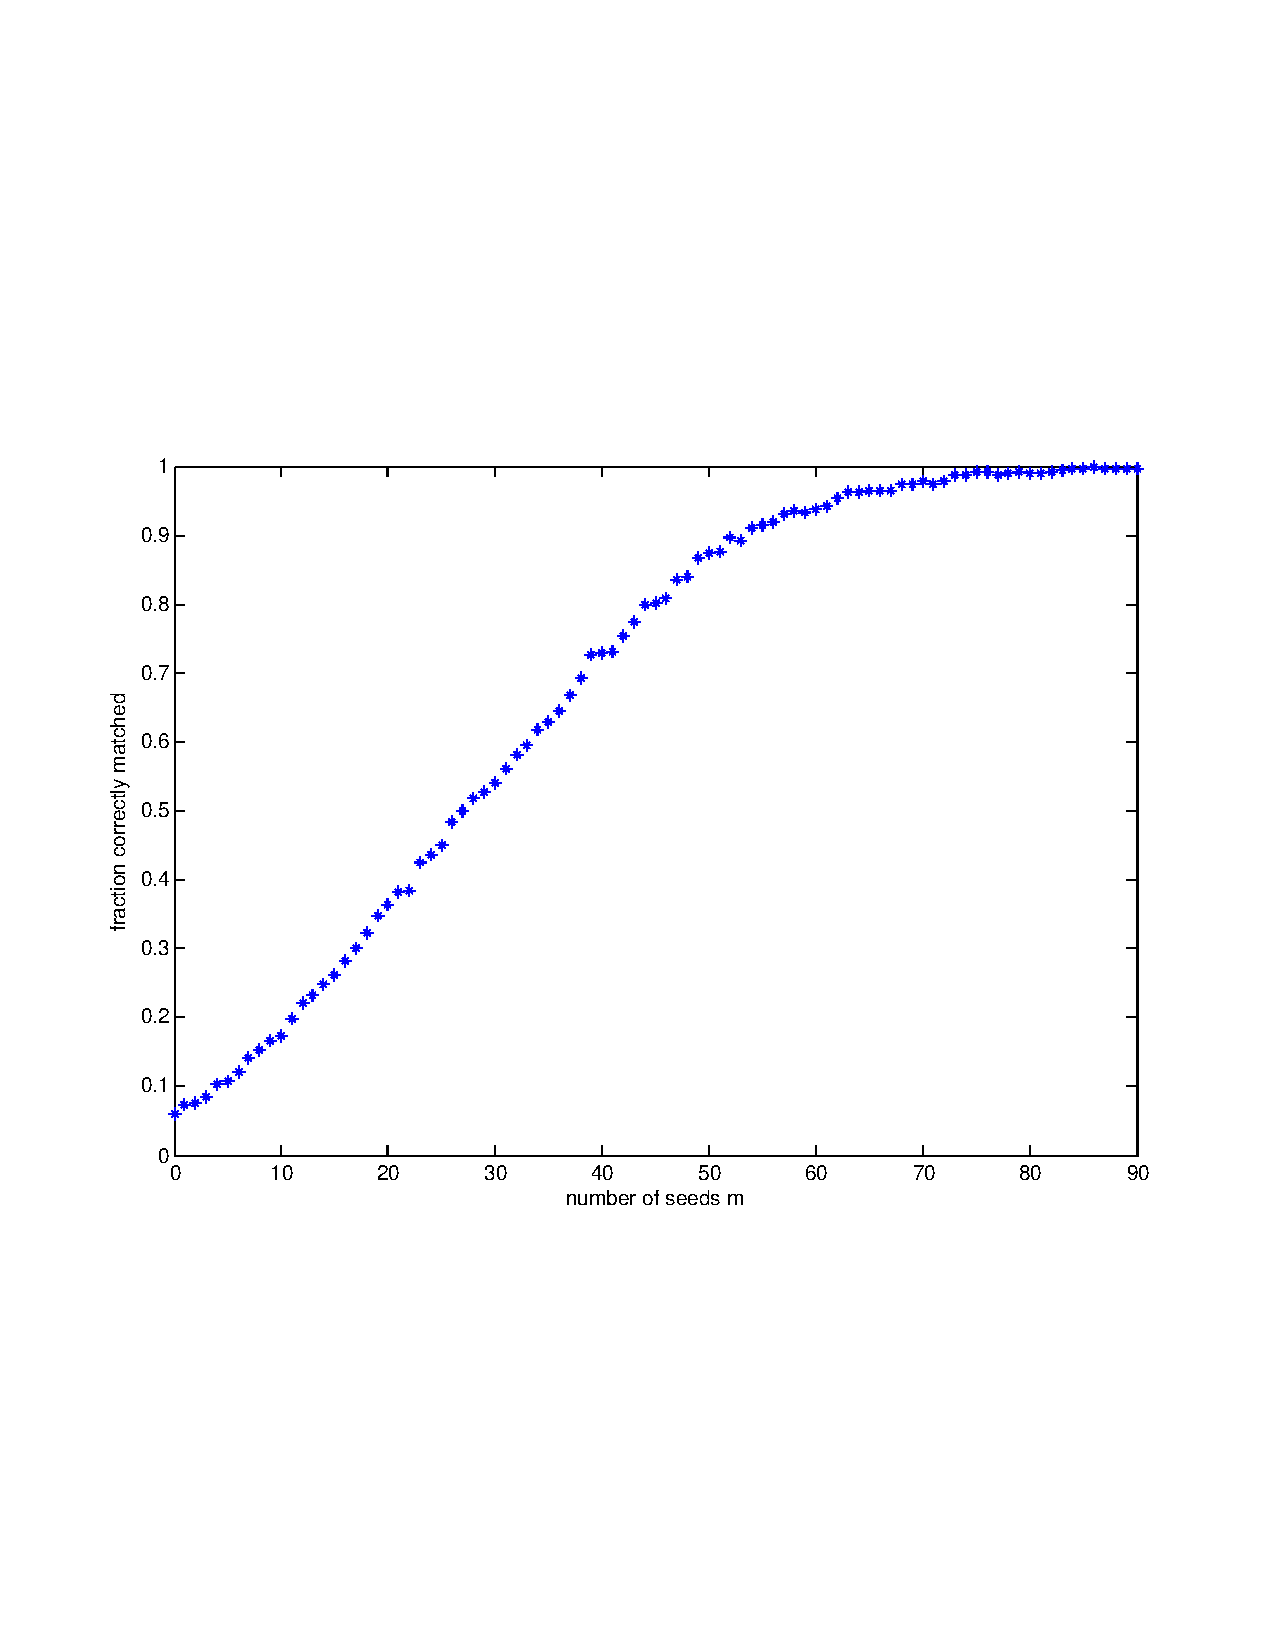
\includegraphics[width=1.2\textwidth]{n30rep65ell1}
  \end{figure}
 \begin{figure}
 \centering
  \caption{Fraction of the $n=30$ nonseeds correctly matched using our $\ell_2$-based algorithm \label{figell2}}
 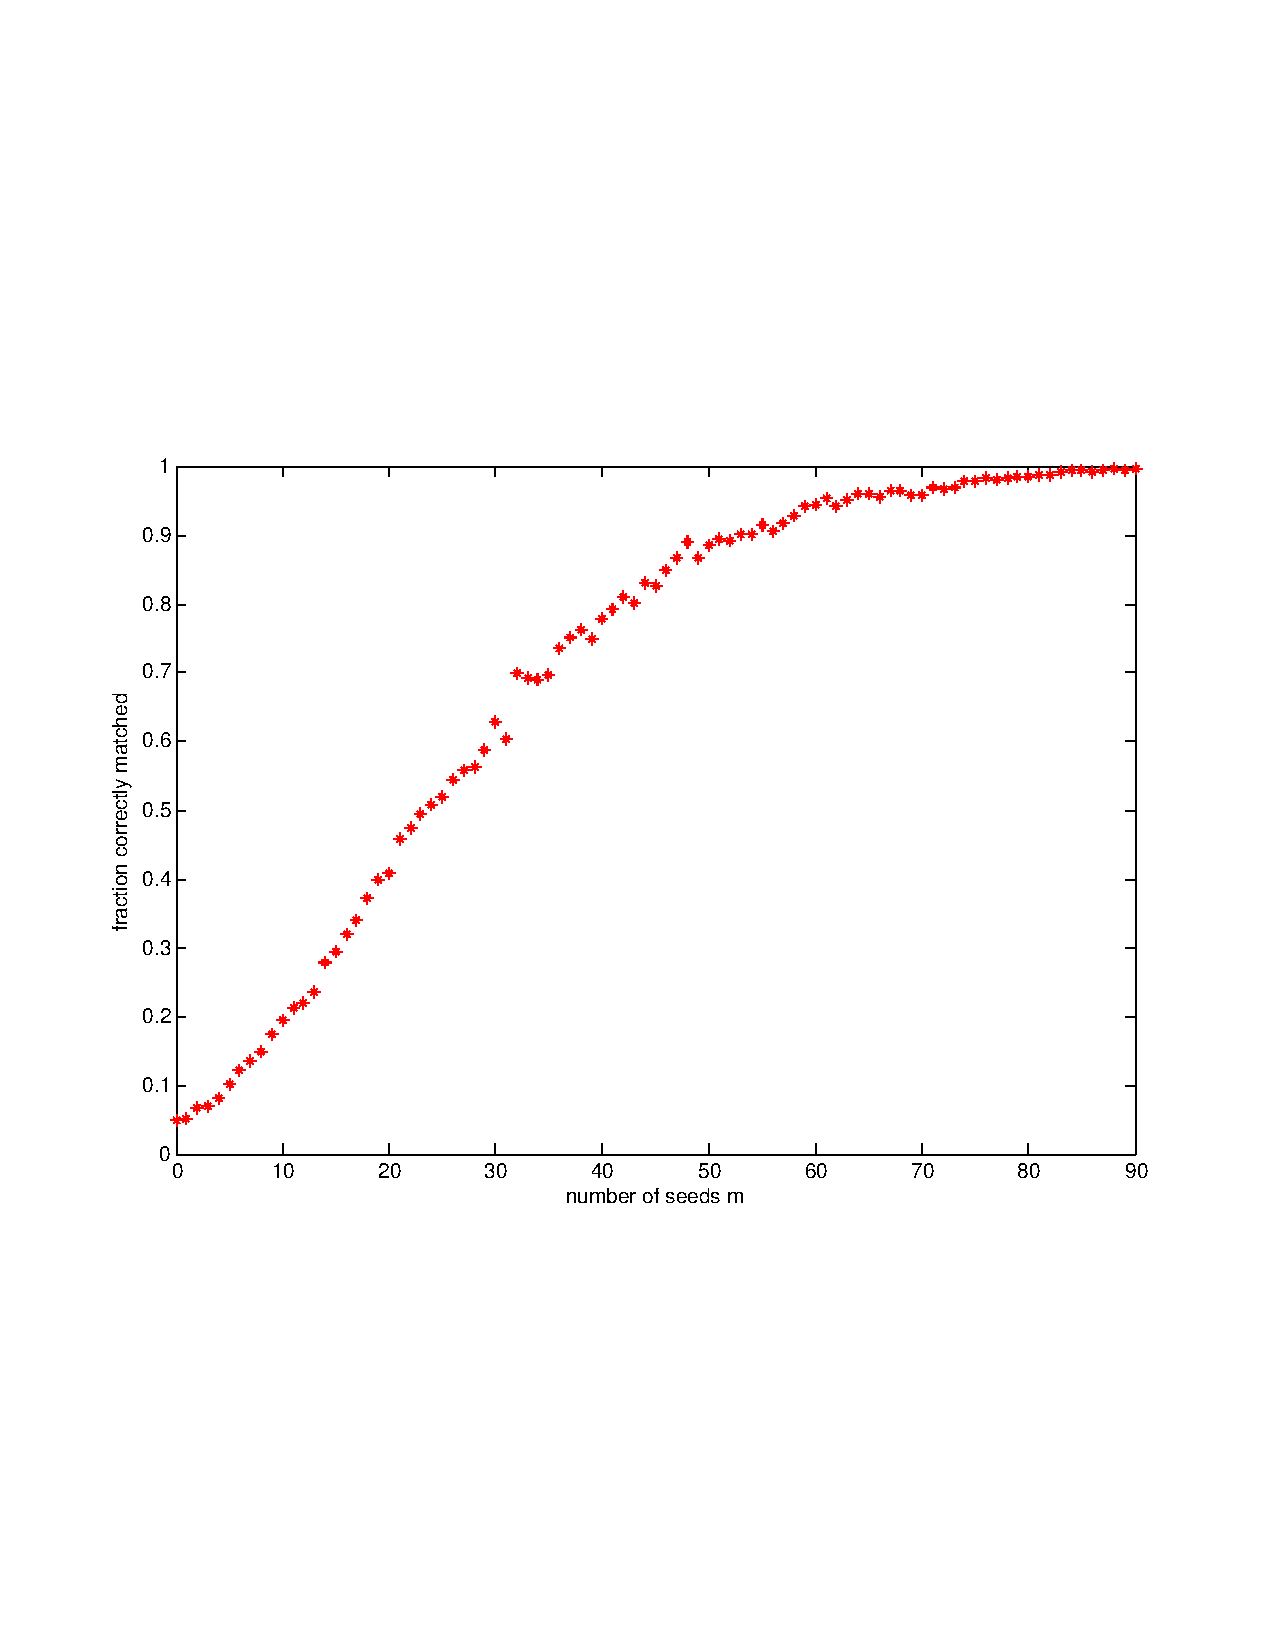
\includegraphics[width=1.2\textwidth]{n30rep65ell2}
\end{figure}


\section{The comparison of rQAP against the alternative formulation rQAP2}
Although the two formulations are equivalent and the global extrema of the two functions are the same, we expect different convergence  properties. In particular the extra terms in the gradient of rQAP2 which vanishes for unitary matrices should act as a random noise. The conclusion of the literature of stochastic optimization  is that, under some conditions, such noise speeds up convergence, by overcoming local extrema. The problem is that, such noise needs to vanish to negligible levels in order for the iterative algorithm to converge. 
The experiment in the last  section was repeated with both rQAP and rQAP2 and the fraction of nonseed vertices correctly matched and the average number of iterations to satisfy a stopping criteria was compared between the two formulations. 

\begin{figure}
 \centering
  \caption{Fraction of the $n=70$ nonseeds correctly matched using our $\ell_2$-based algorithm for rQAP and rQAP2 formulations
 \label{figell2}}
 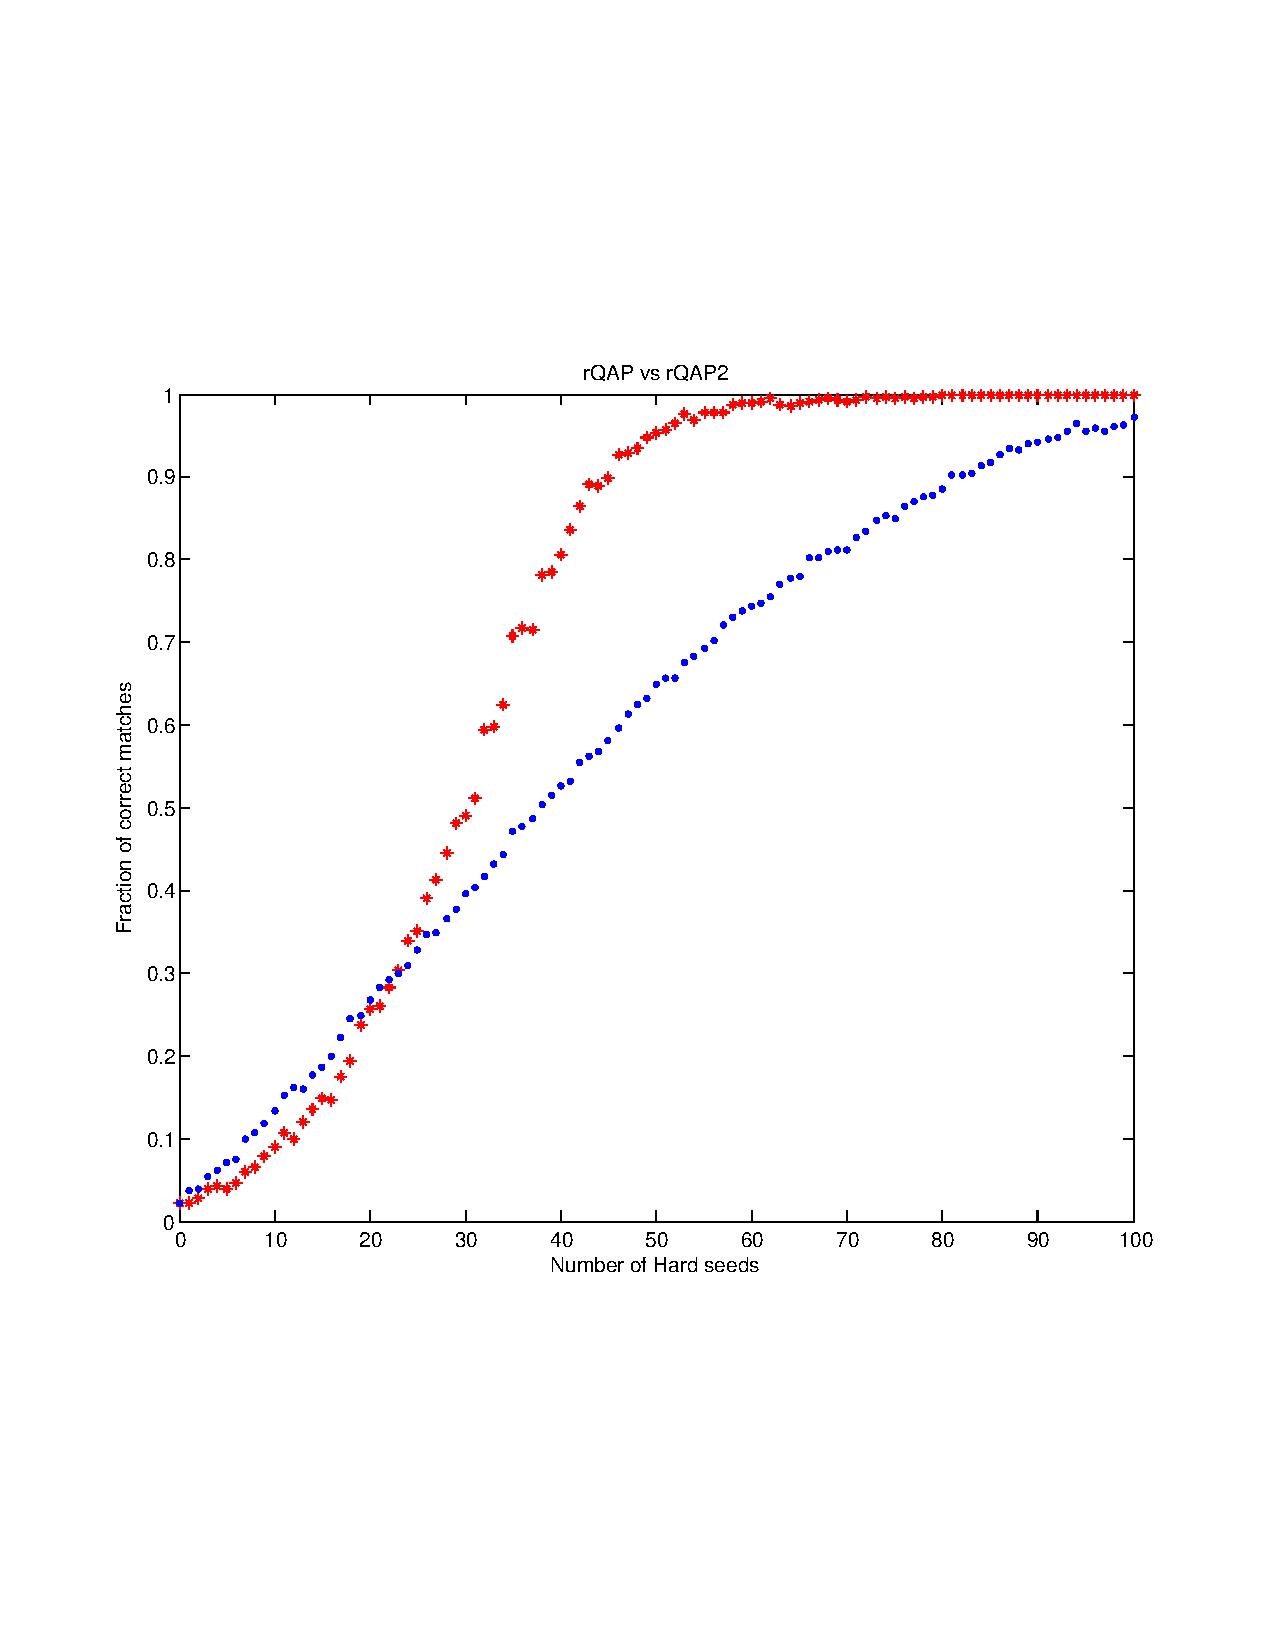
\includegraphics[width=1.2\textwidth]{rQAP_vs_rQAP2-alotmore.pdf}
\end{figure}
Note that for small number of hard seeds $rQAP2$ is slighly better, while for larger number of hard seeds $rQAP$ is clearly better. The average number of iterations of Frank-Wolfe algorithm until termination for the two formulation is as follows,

Our conclusion is that our expectations for the two formulations is warranted, rQAP2   converges slower(or doesn't converge, but stays within the neighborhood of the extrema), whiler rQAP converges in very few steps. When the number of hard seeds is small (which corresponds to lower number of constraints for P and higher incidence of local minima near the true solution. ), rQAP2 is slightly better than rQAP.


A natural follow-up to the previous inquiry is whether one can get the best of both world by making a hybrid of the two formulations: First start with minimizing rQAP2 function, until the current iterate of solution is relatively close to the true solution, and follow with maximizing rQAP function. 

 \section{Alternative methodology of Joint Optimization of Fidelity and Commensurability}
Previous research on embedding of matched objects (whose measurements or  inter-group dissimilarities) has resulted in JOFC approach, which can be summarized as using weighted multidimensional scaling (wMDS) to embed dissimilarities or distances from different conditions/modalities in one joint metric space. The weights in the MDS criteria function controls the tradeoff between  Fidelity (preservation of dissimilarities between unmatched objects of the same condition in the embedding) and preservation of Commensurability  ( preservation of dissimilarities between matched objects of different conditions in the embedding). Since the two graphs are assumed to be isomorphic, the vertices are known to be  matched objects, and embedding graphs is straightforward once a dissimilarity is defined. Therefore JOFC is quite appropriate for this problem. 

\begin{figure}
 \centering
  \caption{Fraction of the $n=70$ nonseeds correctly matched using our $\ell_2$-based algorithm for rQAP and rQAP2 formulations
 \label{figell2}}
 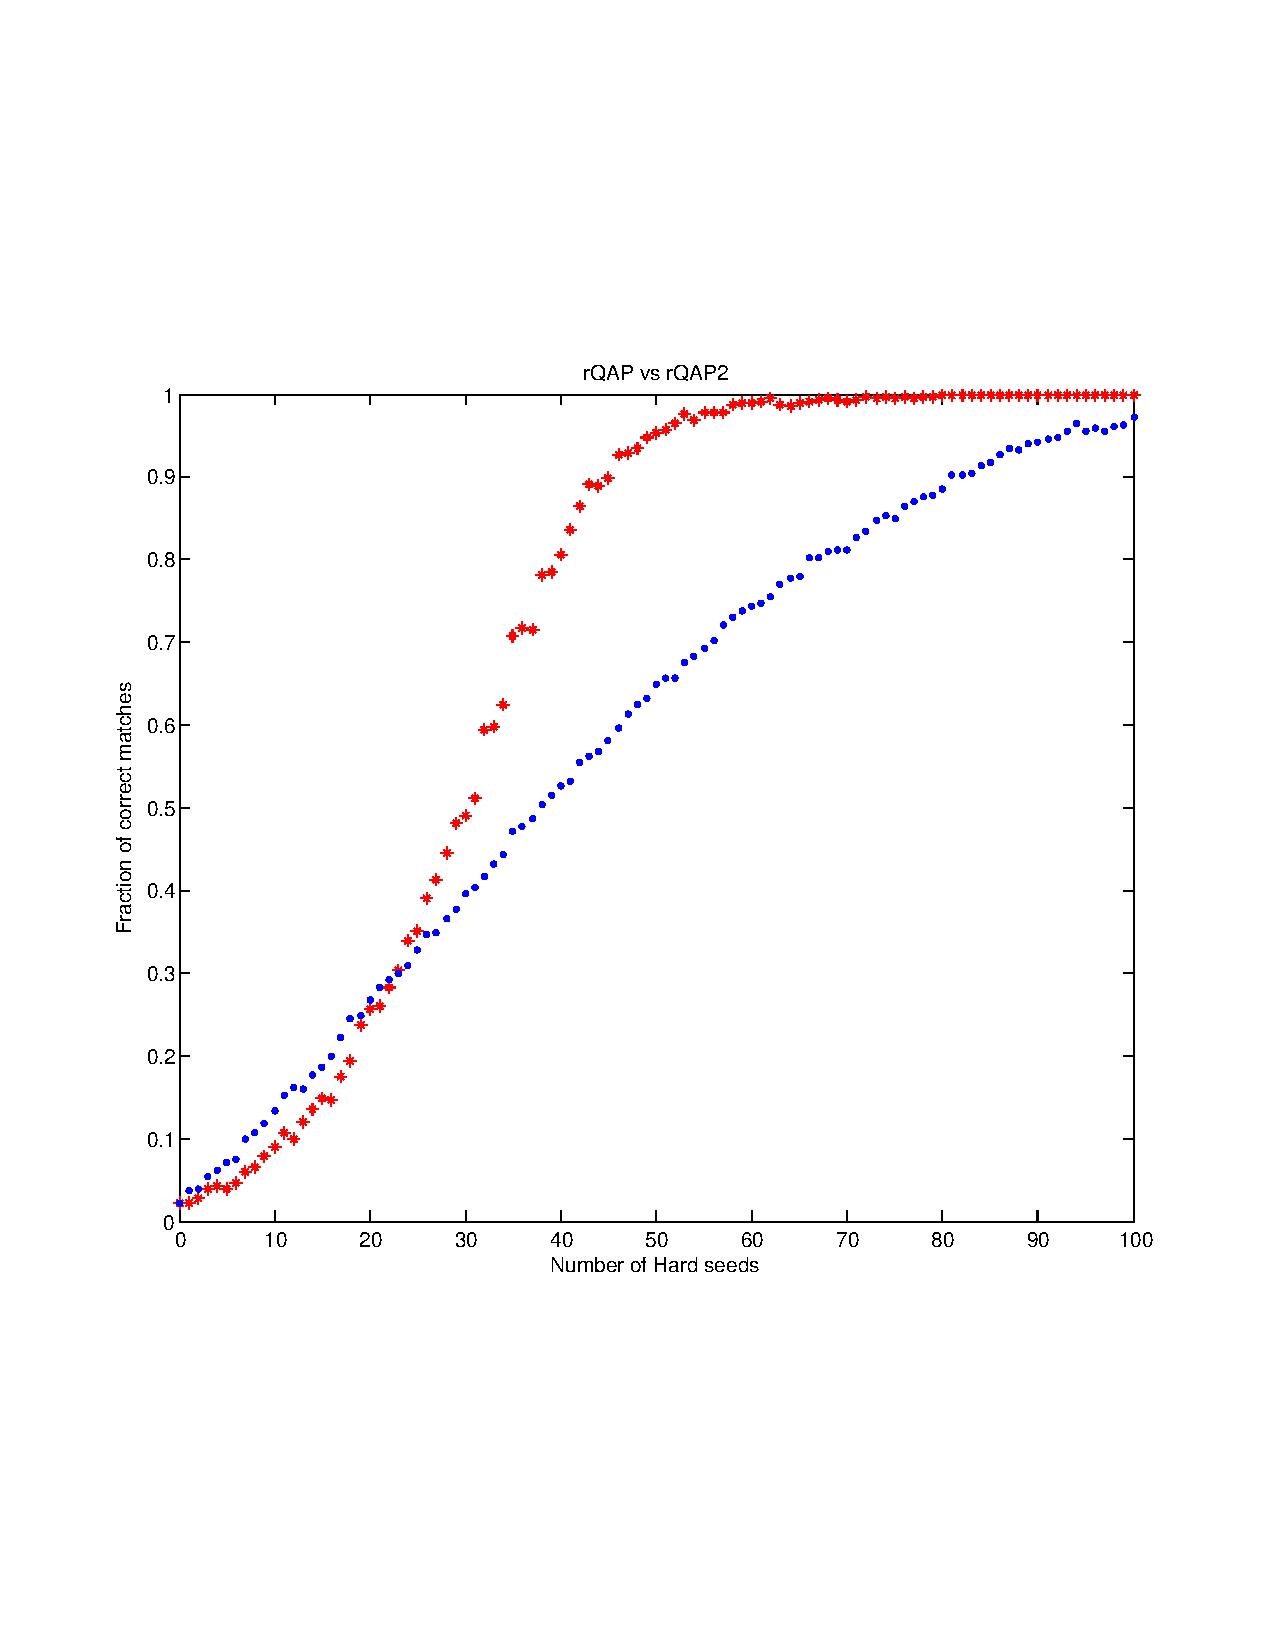
\includegraphics[width=1.2\textwidth]{rQAP_vs_rQAP2-alotmore.pdf}
\end{figure}

\section{seeded graphmatch for group membership}

%Suppose there is a set of so-called ``EnronExecutives" which is
%partitioned into two sets, $W$ and $V$, and there is a set $U$ of
%so-called ``EnronWorkerBees". Let $p$, $q$, and $r$ be fixed real numbers
%in the interval $[0,1]$. A random Enron graph $G$ has vertices $W \cup V \cup U$
%and for every pair of EnronExecutives the probability they form an edge is $p$,
%for every pair of EnronWorkerBees the probability they form an edge is $q$, and for
%every pair consisting of one EnronExecutive and one EnronWorkerBee the
%probability that they form an edge is $r$, every pair of vertices
%independently of every other pair of vertices.
%The graph will be called VU-unlabeled if the vertices of $V \cup U$ have their
%identities removed so that an observer can identify each vertex in $W$ as
%being a member of $W$, but each vertex not in $W$ cannot be
%directly identified as being in $U$ versus being in $V$.

Let $m,n',n''$ be fixed integers, and let $p,q,r$ be fixed real numbers
from the interval $[0,1]$. An {\it Enron adjacency matrix} $A$ is a
random $(m+n'+n'')$-by-$(m+n'+n'')$ adjacency matrix $A$ such that, for
all pairs of distinct $i,j \in \{ 1,2,\ldots,m+n'+n''\}$
(all pairs independently of all other pairs), the entry
$a_{ij}$ has a Bernoulli distribution with parameter $p$, $q$, or $r$
according as both $i$ and $j$ are in $\{ 1,2,\ldots,m+n'\}$,
both $i$ and $j$ are not in $\{ 1,2,\ldots,m+n'\}$, or exactly one of $i$ and $j$
are in $\{ 1,2,\ldots,m+n'\}$.

A {\it graph-to-graph Enron experiment} consists
of realizing two independent Enron adjacency matrices $A$ and $B$, then  discrete-uniformly randomly permuting the last $n'+n''$ vertices of $B$
(ie conformally permuting the last $n'+n''$ rows and the last $n'+n''$
columns of $B$), then doing the seeded graph match procedure from
Section \ref{ell2} using the first $m$ vertices as seeds, and finally
returning the fraction (to be called ``match fraction")
of vertices among $\{ m+1,m+2,m+n' \}$ in $A$
that are matched with vertices that were originally (before permutation)
among $\{ m+1,m+2,m+n' \}$~in~$B$.


A {\it graph-to-parameter} Enron experiment is exactly like a
graph-to-graph Enron experiment except that $A$ is not an Enron
adjacency matrix but, rather, a hollow matrix such that for all
 all pairs of distinct $i,j \in \{ 1,2,\ldots,m+n'+n''\}$
the entry $a_{ij}$ is equal to $p$, $q$, or $r$
according as both $i$ and $j$ are in $\{ 1,2,\ldots,m+n'\}$,
both $i$ and $j$ are not in $\{ 1,2,\ldots,m+n'\}$, or exactly one of $i$ and $j$
are in $\{ 1,2,\ldots,m+n'\}$.

I wrote MATLAB code experimentENgtg.m and experimentENgtp.m to approximate
the mean match fraction for, respectively, graph-to-graph and
graph-to-parameter Enron experiments. The code replicates the experiment
a number of times and returns the sample mean and sample
standard deviation of the match fraction. For 30
replicates in experimentENgtp.m when $m,n',n'',p,q,r$ are respectively
$50,50,100,.5,.5,.4$ we got sample mean match fraction
$.8480$ with sample standard deviation
$.0547$, and with experimentENgtg.m we got sample mean match fraction
$.4473$ with sample standard deviation $.0574$. (Note that the problem
parameters were chosen so that the expected degree of all vertices is the
same, which would pose a extra challenge to some other approaches.)




\end{document}
